\documentclass{JMLFS}

\journal{JMLFS-ID}%Letters in High Energy Physics}
\vol{2020}

%%\publishedtrue%%Uncomment to get following information on first page
\received{xx January 2018}
\published{xx March 2018}

\def\be{\begin{equation}}
\def\ee{\end{equation}}
\def\bea{\begin{eqnarray}}
\def\eea{\end{eqnarray}}
\def\met{\not{\!{\rm E}}_T}
\def\zp{Z^\prime}

\newcommand{\bi}{\bibitem}
\newcommand{\nn}{\nonumber}
\def\BibTeX{\rm B{\sc ib}\TeX}

\begin{document}

\title{Learning Concepts using Deep Neural Networks}

\author{Sunil Kumar Vengalil,\auno{1} and Neelam Sinha\auno{2}}
\address{$^1$International Institute of Information Technology Bangalore}
\address{$^2$International Institute of Information Technology Bangalore}

\begin{abstract}
The ML revolution is in full swing. In fact, the groundwork for it was prepared in the middle of the 20th century, yet, it is only with the ever continuing development of increasingly powerful computers, combined with computational algorithms refined over the past couple of decades, that the world has seen an explosion of applications of ML, in anything from health, to finance down to even autonomous cars!
\end{abstract}

\maketitle

\begin{keyword}
Machine Learning\sep Artificial Intelligence\sep Computer Science
\doi{10.2018/JMLFS000001}
\end{keyword}

\section{Introduction}
One of the major pain points of deep learning models, when used in industry, is the lack of explainability, i.e., they are unable to provide the exact reason for prediction.
One the one hand, researchers build complex ensemble and deep architectures in order to increase the classification accuracy, which results in increased accuracy but the more complex the model is, the more difficult to provide explanations for the predictions.
This trade off between accuracy and explainability of Machine Learning and Deep Learning models is well known \cite{wu2021}.
In many use cases, like medical, customer churn prediction etc, it is as equally important to get an explainable prediction as getting correct predictions.
Sometimes one might even want to compromise with a less accurate model, if it can provide better explanations for the predictions.
This behaviour of Machine Learning and Deep Learning models is in sharp contrast with how humans learn.

Learning in human posses the following special characteristics which the ML and DL models starve to achieve.
\begin{enumerate}

\item When humans learns something new, over a period of time they gradually  1)internalize the concepts 2) abstracts the concepts and 3) reuse the concepts in related tasks- all these accomplished usually from a very few samples \cite{lake2015}.

\item The learned concepts are more generic as opposed the predictions, they make using the concept, in a particular scenario.
Each scenario might be different, but the concept used to make an inference will be same.
In other words, they use the same concept to make predictions for different input scenarios i.e the mapping between concept and scenario is one to many.

\item Humans can always provide an explanation for what they predict using the concepts they learned (Irrespective of the fact that the prediction might be wrong).

\end{enumerate}
In this article, we examine how such behaviours can be incorporated into deep learning models.
Explainability in DL models is something which has been actively researched and many approaches has been suggested in the literature in last decade\cite{linardatos2021}.
See section \ref{lit_survey_explainability} for an extensive literature survey of explainability on deep learning models.
However, our approach is not just to inject explainability into a trained deep learning model.
We rather, focus on how the underlying model can learn \textbf{generalized concepts}  which are used to make predictions.


There has been previous studies \cite{mr01} on developing models that learn concept and use the learned concepts in a human like manner using Baysean Probabilistic Language \cite{}.

In this article we report results of experiemnts performed on image datasets of varying complexity starting from MNIST, CIFAR-10, CIFAR-100 and Cat Vs Dog datasets.
We propose an approach for learning classification and segmentation tasks while the model also learns the concepts associated with the dataset/task.

\section{Related Work}
\subsection{Explainability in Deep Learning Models}\label{lit_survey_explainability}
\subsection{Concept Learning}
\subsection{Semi-supervised Learning}

\section{{ PROPOSED METHOD}}

\subsection{Overview of Approach}

\subsection{Datasets}

\subsection{Primary Visual Concepts}
\subsection{Composition of concepts}
%\subection{Network Architecture, Loss function and Training}

\begin{itemize}
\item  {\tt add tetex} allows access on {\tt unity} to a
comprehensive distribution of \LaTeX\, called {\tt tetex} (optional)

\item  Here, {\tt ghostview} is used to view the
final document

\item  Using instead {\tt dvips -P pdf latex1} creates a postscript
file that is optimal if the a pdf file is to be created, e.g.,
using acrobat distiller or the {\tt ps2pdf} utility
\end{itemize}
\begin{verbatim}
stat% distill latex1.ps   OR  stat% ps2pdf latex1.ps
\end{verbatim}

{\bf Structure of a {\tt .tex} file:}
\begin{itemize}
\item  {\sl Preamble}
\begin{itemize}
\item Specify {\sl document class} (article, report, book,
letter, etc.)
\item Add any ``{\sl packages}'' used (e.g., to import
graphics, create headers and footers, etc.)

\item Specify {\sl margins}, {\sl indentation},
{\sl spacing}, etc.

\item Define ``{\sl new commands}'' (coming up\ldots)
\end{itemize}

\item  {\sl Document body}
\begin{itemize}
\item The actual document content
\end{itemize}
\end{itemize}

{\bf Fun facts:}
\begin{itemize}
\item  \% symbol is used to document the file or ``{\sl
comment out}'' text; anything to the right of a \% does not appear
in the document

\item  \LaTeX\, commands start with \verb+\+

\item  \LaTeX\, is {\sl case sensitive}

\end{itemize}

{\bf For example:} Here is a sample preamble and document body
for an article (See the web page for a full template file)


\begin{small}
\addtolength{\baselineskip}{-1.5ex}
\begin{verbatim}
\documentclass[12pt]{article} % type size: also 10pt or 11pt

% commands to set margins and spacing -- all have defaults

\setlength{\textheight}{9in}    % height of text on a page
\setlength{\textwidth}{6.5in}   % width of text on a page
\setlength{\parskip}{2.3ex}     % space between paragraphs

% commands to invoke packages

\usepackage{graphicx,psfig,epsf}    % no limit to how many

% user-defined newcommands

\newcommand{\betahat}{\hat{\beta}}  % more on this shortly

%  start of document body


\begin{document}

\section{Introduction}              % sectioning command

This is the introduction...

\end{document}
\end{verbatim}
\addtolength{\baselineskip}{1.5ex}
\end{small}

{\bf Syntax:}  Some commands have arguments in braces \{\,\},
some do not

\subsection*{Some commands with no argument:}
\begin{verbatim}
\ldots, \dag, \ddag, \%, \&, \#, \{ \}, \today, \LaTeX
\end{verbatim}
\ldots, \dag, \ddag, \%, \&, \#, \{ \}, \today, \LaTeX

{\bf Commands with arguments:} \verb+\setlength{ ... }+,\\
\verb+\section{ ... }+, \verb+\subsection{ ... }+, \verb+\hspace{ ... }+,\\
\verb+\vspace{ ... }+




\section{{ MODES AND ENVIRONMENTS}}

{\bf Modes:} At any point in a \LaTeX\, file, there is a current
``{\sl mode}'' in effect
\begin{itemize}
\item  {\sl Paragraph mode} -- the default text mode, with
line wrap.  A space between lines signals the start of a new paragraph

\item  {\sl Math mode} -- math symbols and commands may be used,
and mathematical expressions result

\item  {\sl LR mode} -- ``left-to-right'' mode, lines do not
automatically wrap around
\end{itemize}

{\bf Note on math mode:} Math symbols and commands only work in
math mode; if they are used in other modes, an {\sl error}
will result

{\bf Environments:} Often, there is also an {\sl environment}
in effect that determines how material is displayed -- the basic
structure is

\begin{verbatim}
\begin{environment-name}
...
\end{environment-name}
\end{verbatim}

{\bf For example:} The {\tt math} environment
\begin{verbatim}
the linear model
\begin{math}Y = X\beta + \epsilon\end{math}.
\end{verbatim}
the linear model $Y = X\beta + \epsilon$.
\begin{itemize}
\item  The popular shortcuts are to use \verb+$ ... $+ or \verb+\( ... \)+, e.g.
\end{itemize}
\begin{verbatim}
the linear model $Y = X\beta + \epsilon$.
\end{verbatim}

{\bf For example:} Creating a numbered list
\begin{verbatim}
\begin{enumerate}
\item This is the first entry
\item This is the second entry
\item This is the third entry
\end{enumerate}
\end{verbatim}

\begin{enumerate}
\item This is the first entry
\item This is the second entry
\item This is the third entry
\end{enumerate}

{\bf Some popular environments:}
\begin{tabular}{lll}
Environment & Mode & Description \\*[-0.05in] \hline
{\tt math} & math & in-text mathematical expressions \\*[-0.05in]
{\tt displaymath} & math & displayed mathematical expressions \\*[-0.05in]
{\tt equation} & math & displayed expressions w/ line number \\*[-0.05in]
{\tt eqnarray} & math & lines up equal signs, line numbers \\*[-0.05in]
{\tt eqnarray*} & math & lines up equal signs, no line numbers \\*[-0.05in]
{\tt array} & math & matrices and arrays \\*[-0.05in] \hline
{\tt itemize} & paragraph & list with bullets \\*[-0.05in]
{\tt enumerate} & paragraph & list with numbers \\*[-0.05in]
{\tt description} & paragraph & list with indentation \\*[-0.05in] \hline
{\tt tabular} & LR & align text in columns \\*[-0.05in]
{\tt table} & paragraph & number and position table \\*[-0.05in]
{\tt figure} & paragraph & number and position figure \\*[-0.05in] \hline
{\tt center} & paragraph & center text \\*[-0.05in]
{\tt mbox} & LR & write text while in math mode \\*[0.1in]
\end{tabular}

{\bf Math:} \LaTeX\, is {\sl tailor-made} for writing involving
high mathematical content! And it's easy!
\begin{itemize}
\item  {\sl Subscripts, superscripts, roots}
\begin{verbatim}
e^y, x_{ij}, \sqrt{x+y}, \sum^n_{i=1}
\end{verbatim}
$e^y, x_{ij}, \sqrt{x+y}, \sum^n_{i=1}$
\item  {\sl Greek}
\begin{verbatim}
\alpha,\beta,\gamma,\delta,\epsilon,\eta,\theta,
\lambda
\end{verbatim}
$\alpha,\beta,\gamma,\delta,\epsilon,\eta,\theta,\lambda$
\begin{verbatim}
\Gamma,\Delta,\Theta,\Lambda,\Omega,\Sigma
\end{verbatim}
$\Gamma,\Delta,\Theta,\Lambda,\Omega,\Sigma$

\item  {\sl Roofs}
\begin{verbatim}
\hat{\alpha},\tilde{\alpha},\dot{x},\overline{x},
\bar{x}
\end{verbatim}
$\hat{\alpha},\tilde{\alpha},\dot{x},\overline{x},\bar{x}$
\end{itemize}

{\bf Math, continued:}
\begin{itemize}
\item  {\sl Binary operations}
\begin{verbatim}
\pm,\times,\div,\cup,\otimes
\end{verbatim}
$\pm,\times,\div,\cup,\otimes$

\item  {\sl Relation symbols}
\begin{verbatim}
\leq,\subset,\in,\geq,\equiv,\sim,\approx,\neq,\perp
\end{verbatim}
$\leq,\subset,\in,\geq,\equiv,\sim,\approx,\neq,\perp$

\item  {\sl Arrows}
\begin{verbatim}
\rightarrow,\Leftarrow,\Leftrightarrow,\uparrow
\end{verbatim}
$\rightarrow,\Leftarrow,\Leftrightarrow,\uparrow$

\item  {\sl Miscellaneous}
\begin{verbatim}
\forall,\exists,\Re,\sum,\prod,\int
\end{verbatim}
$\forall,\exists,\Re,\sum,\prod,\int$
\end{itemize}

\vskip11.3pc
{\bf Math, continued:}  {\tt textstyle} vs. {\tt displaystyle}
\begin{itemize}
\item  Math {\sl displayed} as equations may be carried out
using the {\tt displaymath}, {\tt equation}, {\tt eqnarray*}, {\tt
eqnarray} environments

\item  {\sl Shortcuts} when equations are {\sl not
numbered}: \verb+$$ ... $$+ or \verb+\[ ... \]+; e.g.,
\begin{verbatim}
$$\sum^n_{i=1} x_i^2 (Y_{ij}-z_i \beta)$$
\end{verbatim}
$$\sum^n_{i=1} x_i^2 (Y_{ij}-z_i \beta)$$

\item  Some symbols appear {\sl differently} depending on
whether they are in the text or displayed; e.g.,
\begin{verbatim}
$\sum^n_{i=1}$      VS.  $$\sum^n_{i=1}$$
\end{verbatim}
$\sum^n_{i=1}\hspace{0.1in}\mbox{\tt VS.}\hspace{0.1in}
\displaystyle{\sum^n_{i=1}}$

\item  Can be {\sl overridden} with \verb+textstyle{  }+
and\\ \verb+\displaystyle{  }+
\end{itemize}

{\bf Math, continued:}
\begin{itemize}
\item  {\sl Products, integrals, unions}
\begin{verbatim}
$$\prod^n_{j=1},\hspace{0.1in} \int^\infty_t f(u) du,
\hspace{0.1in}\bigcup_{A: A \in \Omega}$$
\end{verbatim}
$$\prod^n_{j=1},\hspace{0.1in} \int^\infty_t f(u) du, \hspace{0.1in}
\bigcup_{A: A \in \Omega}$$

\item  {\sl Special functions}
\begin{verbatim}
$\exp(x), \log y, \sin(k\pi), \min_x f(x)$
\end{verbatim}
$\exp(x), \log y, \sin(k\pi), \min_x f(x)$

\item  Fractions, partial derivatives
\begin{verbatim}
$$\frac{\exp(x^T \beta)}{1+\exp(x^T \beta)},
\frac{\partial u}{\partial x}$$
\end{verbatim}
$$\frac{\exp(x^T \beta)}{1+\exp(x^T \beta)}, \frac{\partial u}{\partial x}$$
\end{itemize}

{\bf Note:} Use \verb+\displaystyle+ for fractions; otherwise
they are too small

{\bf Math, continued:} There are different ways to
present math in {\bf boldface}; here are two
\begin{itemize}
\item  \verb+$\mbox{\boldmath $X$}$+, output $\mbox{\boldmath $X$}$\\
\verb+$\mbox{\boldmath $\Sigma$}$+, output  $\mbox{\boldmath $\Sigma$}$

\item  \verb+$\mathbf{X}$, $\mathbf{\Sigma}$+ \\
$\mathbf{X}$, $\mathbf{\Sigma}$
\end{itemize}

{\bf Math, continued:} {\tt array} and {\tt eqnarray} environments
\begin{itemize}
\item  $(2 \times 3)$ {\sl matrix}:
\begin{verbatim}
   \left( \begin{array}{ccc}
      x_{11} & x_{12} & x_{13}\\
      x_{21} & x_{22} & x_{23}
          \end{array} \right)
\end{verbatim}
$$\left( \begin{array}{ccc}
x_{11} & x_{12} & x_{13} \\
x_{21} & x_{22} & x_{23} \end{array} \right)$$

\item  {\sl Determinant} of $(2 \times 2)$ matrix:
\begin{verbatim}
   \left| \begin{array}{cc}
      a_{11} & a_{12} \\
      a_{21} & a_{22} \end{array} \right|
\end{verbatim}
$$\left| \begin{array}{cc}
   a_{11} & a_{12} \\
   a_{21} & a_{22} \end{array} \right|$$
\end{itemize}

{\bf Math, continued:} {\tt array} and {\tt eqnarray} environments
\begin{itemize}
\item  {\sl Braces}
\begin{verbatim}
x = \left\{ \begin{array}{l}
     \sin x \mbox{ if } y<3, \\
     \cos x \mbox{ if } y \geq 3
            \end{array} \right.
\end{verbatim}
$$ x = \left\{ \begin{array}{l} \sin x \mbox{ if } y<3, \\
                  \cos x \mbox{ if } y \geq 3 \end{array} \right.$$

\item  {\sl Binomial coefficients}:
\verb+\left( \begin{array}{c}N \\ y+
\verb+ \end{array} \right)+
$$\left( \begin{array}{c}N \\ y \end{array} \right)$$
\end{itemize}

{\bf Math, continued:} {\tt array} and {\tt eqnarray} environments
\begin{itemize}
\item  {\sl Equation with several lines, = signs lined up}
\end{itemize}
{\footnotesize\begin{verbatim}
\begin{eqnarray*}
\Delta_i & = & \sum_j \sum_{k \neq j} \mbox{Corr}(Y_{ij},Y_{ik}) \\
 & = & \sum_j \sum_{k \neq j} \rho_i^{\parallel j-k \parallel} \\
 & = & \frac{2 \rho_i}{1-\rho_i} \left\{ n_i-1 -
          \frac{\rho_i(1-\rho_i^{n_i-1})}{1-\rho_i} \right\}
\end{eqnarray*}
\end{verbatim}}
\begin{eqnarray*}
\Delta_i & = & \sum_j \sum_{k \neq j} \mbox{Corr}(Y_{ij},Y_{ik}) \\
   & = & \sum_j \sum_{k \neq j} \rho_i^{\parallel j-k \parallel} \\
   & = & \frac{2 \rho_i}{1-\rho_i} \left\{ n_i-1 -
          \frac{\rho_i(1-\rho_i^{n_i-1})}{1-\rho_i} \right\}
\end{eqnarray*}



{\bf The {\tt tabular} environment:}
\begin{itemize}
\item  As with {\tt array}, separate {\sl elements} with \&,
make {\sl new line} with \verb+\\+
\item  Specify {\sl number of columns} and type of {\sl
justification} at top, add {\sl vertical} and {\sl horizontal}
lines
\end{itemize}
\begin{small}
\begin{verbatim}
\begin{tabular}{c|rr}
 & \multicolumn{2}{c}{Results} \\
Parameter & \multicolumn{1}{c}{Bias} & \multicolumn{1}{c}{SE} \\
\hline
$\beta_0$ & $-$0.030 & 0.12 \\
$\beta_1$ & 0.002 & 0.07
\end{tabular}
\end{verbatim}
\end{small}
\begin{tabular}{c|rr}
 & \multicolumn{2}{c}{Results} \\
 Parameter & \multicolumn{1}{c}{Bias} & \multicolumn{1}{c}{SE} \\ \hline
 $\beta_0$ & $-$0.030 & 0.12 \\
 $\beta_1$ & 0.002 & 0.07
\end{tabular}


\newcommand{\bbeta}{\mbox{\boldmath $\beta$}}
\newcommand{\betahatj}{\widehat{\bbeta}_j}
\newcommand{\var}{\mbox{var}}
\newcommand{\sumjn}{\sum^n_{j=1}}

\section{{ NEWCOMMANDS}}
{\bf Motivation:} In technical typing, the same (nasty)
expression may appear {\sl frequently}
\begin{itemize}
\item  A {\tt newcommand} is like a ``{\sl shortcut}'' to produce
the expression easily
\item   \verb+\newcommand{keyword}{text}+
\item  A {\tt newcommand} declaration may appear {\sl anywhere}
 in a \LaTeX\, source file (preamble or body) and is defined thereafter
\item  A {\tt newcommand} {\tt keyword} may {\sl not} contain
numbers
\end{itemize}



{\bf Examples:} Some {\tt newcommand} definitions and their usage
\begin{verbatim}
\newcommand{\bbeta}{\mbox{\boldmath $\beta$}}
\newcommand{\betahatj}{\widehat{\bbeta}_j}
\newcommand{\var}{\mbox{var}}
\newcommand{\sumjn}{\sum^n_{j=1}}
\end{verbatim}
\begin{itemize}
\item  Note that a {\sl previously-defined} {\tt newcommand} may be
used in defining a {\sl new} {\tt newcommand}
\end{itemize}

\begin{verbatim}

               $$\sumjn \var(\betahatj)$$
\end{verbatim}
$$\sumjn \var(\betahatj)$$




\section{{ CROSS REFERENCES}}
{\bf Advantage:} A {\sl built-in} feature of \LaTeX\,
is that it {\sl automatically} keeps track of sections,
numbered equations, pages, and so on
\begin{itemize}
\item  Sections, equations, tables, figures, pages etc.
may be {\sl labeled} and referred to by the label
\item  If new labeled entities are added, \LaTeX\, {\sl renumbers}
them automatically
\item  It is even possible to generate a {\sl table of
contents} and {\sl index} for a document
\item  To set up cross references correctly, must process
a document {\sl twice}
\end{itemize}
\begin{small}
\verb+      \LaTeX Warning: Label(s) may have changed.+\\
\verb+         Rerun to get cross-references right.+
\end{small}

{\bf Examples:}
\begin{itemize}
\item  Numbered equation
\begin{verbatim}
\begin{equation}
\var(\alpha) = \sumjn \var(\betahatj)
\label{eq:alpha}
\end{equation}

In equation~\ref{eq:alpha}, we see that...
\end{verbatim}
\end{itemize}

{\bf Examples, continued:}
\begin{itemize}
\item  Section label
\begin{verbatim}
\section{Introduction}
\label{s:intro}

...As discussed in Section~\ref{s:intro},
kurtosis...
\end{verbatim}

\item  Page label
\begin{verbatim}
Thus, we see that calculation of the variance is
straightforward \label{p:var}


...On page~\pageref{p:var}, the variance
 calculation...
\end{verbatim}
\end{itemize}

\section{{ PACKAGES}}
{\bf Useful utilities:} \LaTeX\, is much more {\sl powerful}
than the intrinsic features would suggest
\begin{itemize}
\item  A {\sl huge} user community

\item  Contributed {\sl document classes}, ``{\sl add-ons}''
to allow different capabilities and customization

\item  ``{\sl Packages}''

\item  Define new commands, syntax, etc.

\item  Visit {\tt CTAN} (see slide~\pageref{slide:ref})
\end{itemize}

{\bf Example:} {\tt fancyheadings.sty} -- make ``{\sl fancy}''
document {\sl headers} and {\sl footers}
\begin{itemize}
\item  In preamble
\begin{verbatim}
\usepackage{fancyheadings}
\lhead{\footnotesize \bf CHAPTER \thesection}
\rhead{\footnotesize \bf ST 762, M. DAVIDIAN}
\cfoot{\footnotesize PAGE \rm\thepage}
\end{verbatim}

\item  See {\tt http://www.stat.ncsu.edu/$\sim$st762\_info/} for results
\end{itemize}

{\bf Example:} {\tt shadow.sty} -- make ``{\sl shadowboxes}''
\begin{itemize}
\item  In preamble
\begin{verbatim}
\usepackage{shadow}

\shabox{This stuff}
\end{verbatim}
{This stuff}%\shabox shashi
\end{itemize}

{\bf In addition:} There are also user-defined, alternative {\sl
document classes}
\begin{itemize}
\item  {\sl Journals}, {\sl book publishers} may have their
own class to create articles, pages with a specific format
\end{itemize}

\subsection*{Dissertations:} At NCSU, dissertations may be created in
\LaTeX\, using special a special style; to learn more, visit

\begin{small}
\begin{verbatim}
http://www2.acs.ncsu.edu/grad/ETD/tutorial/latex.htm

http://www.stat.ncsu.edu/computing/howto/latex/
          session_2/session2.html
\end{verbatim}
\end{small}

\section{{ IMPORTING GRAPHICS}}
\subsection*{Numerous options:} We discuss three of these
\begin{itemize}
\item  {\tt psfig} -- \verb+\usepackage{psfig}+
\begin{verbatim}
\psfig{figure=dental.ps,height=2.5in}
\end{verbatim}
\end{itemize}

\begin{itemize}
\item  {\tt epsf} -- \verb+\usepackage{epsf}+
\begin{verbatim}
\epsfysize=2.5in
\epsfbox{dental.ps}
\end{verbatim}
\end{itemize}

\begin{itemize}
\item  {\tt graphicx} -- \verb+\usepackage{graphicx}+
\item  Can also import other formats (pdf, jpg, etc)
\begin{verbatim}
\includegraphics[height=2.5in]{dental.ps}
\end{verbatim}
\end{itemize}

\section{{ TABLES AND FIGURES}}
\subsection*{Two standard \LaTeX\, environments:} {\tt table} and {\tt figure}
\begin{itemize}
\item  Automatically {\sl numbers} tables and figures
\item  Allow tables and figures to be formatted and {\sl referenced}
within a document
\item  Allow {\sl captions}
\end{itemize}

\begin{small}
\begin{verbatim}
\begin{table}[h!]
\tbl{Results of the simulation.\label{t:simresults}}{%
\begin{tabular}{crr}
\toprule
 & \multicolumn{2}{c}{Results} \\
 Parameter & \multicolumn{1}{c}{Bias} &
                              \multicolumn{1}{c}{SE} \\
\colrule
 $\beta_0$ & 0.030 & 0.12 \\
 $\beta_1$ & 0.002 & 0.07\\
 \botrule
\end{tabular}}
\end{table}
\end{verbatim}
\end{small}

\begin{table}[h!]
\tbl{Results of the simulation.\label{t:simresults}}{%
\begin{tabular}{crr}
\toprule
 & \multicolumn{2}{c}{Results} \\
 Parameter & \multicolumn{1}{c}{Bias} & \multicolumn{1}{c}{SE} \\
\colrule
 $\beta_0$ & 0.030 & 0.12 \\
 $\beta_1$ & 0.002 & 0.07\\
 \botrule
\end{tabular}}
\end{table}

\begin{itemize}
\item  Reference -- \verb+In Table~\ref{t:simresults},+\\ \verb+we see that...+
\item  In Table~\ref{t:simresults}, we see that\ldots
\end{itemize}

\begin{verbatim}
\begin{figure}
\centering
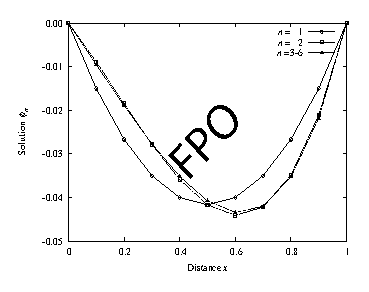
\includegraphics[height=2in]{fpo.eps}
\caption{The dental data of Pothoff and Roy.}
\label{f:dental}
\end{figure}
\end{verbatim}

\begin{figure}[h!]
\centering
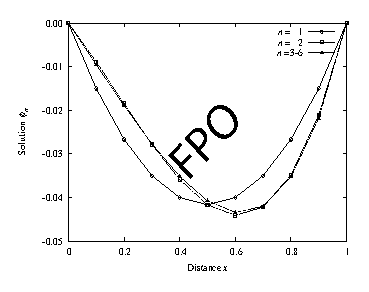
\includegraphics[height=2in]{fpo.eps}
\caption{The dental data of Pothoff and Roy.}
\label{f:dental}
\end{figure}

\subsection*{Useful package:} {\tt subfigure} -- \verb+\usepackage{subfigure}+
\begin{itemize}
\item  Create a ``{\sl multipanel}'' figure from several
files with each panel labeled
\end{itemize}
\begin{small}
\begin{verbatim}
\begin{figure}
    \centering \subfigure[]{
        \includegraphics[width=1.5in]{dental.ps}}
        \hspace*{0.1in}
        \subfigure[]{
        \includegraphics[width=1.5in]{dental.ps}}
\caption{(a) The dental data of Pothoff and Roy.  (b) The dental
data of Pothoff and Roy, again.}
\label{f:dental2}
\end{figure}
\end{verbatim}
\end{small}

\section{{ PICTURES}}
\subsection*{\LaTeX\ can ``draw'':}
\begin{itemize}
\item {\tt picture} environment
\item The following is a {\sl simple} picture --
circles, curves, ovals, etc are also possible (see the documentation)
\end{itemize}

\subsection*{Two-compartment open model with IV administration:}
\vspace{0.5in}
\begin{center}
\setlength{\unitlength}{0.75in}
\begin{picture}(5,1)
\put(0.5,0.5){\framebox(1.5,1){$C(t)$}}
\put(2,1.25){\vector(1,0){0.5}}
\put(2.25,1.35){\makebox(0,0){$k_{12}$}}
\put(2.5,0.75){\vector(-1,0){0.5}}
\put(2.25,0.85){\makebox(0,0){$k_{21}$}}
\put(2.5,0.5){\framebox(1.5,1){$C_{tis}(t)$}}
\put(0.25,1){\makebox(0,0){$D:$}}
\put(1.25,0.5){\vector(0,-1){0.3}}
\put(1.35,0.35){\makebox(0,0){$k_{e}$}}
\end{picture}
\begin{eqnarray*}
\frac{dC(t)}{dt} = k_{21}C_{tis}(t)-k_{12}C(t)-k_{e}C(t),\\
\frac{C_{tis}(t)}{dt}=k_{12}C(t)-k_{21}C_{tis}(t),\mbox{  }
C_{tis}(0)=0
\end{eqnarray*}
\end{center}

\subsection*{Picture was made with:}
\begin{verbatim}
\setlength{\unitlength}{1in}
\begin{picture}(5,1)
\put(0.5,0.5){\framebox(1.5,1){$C(t)$}}
\put(2,1.25){\vector(1,0){0.5}}
\put(2.25,1.35){\makebox(0,0){$k_{12}$}}
\put(2.5,0.75){\vector(-1,0){0.5}}
\put(2.25,0.85){\makebox(0,0){$k_{21}$}}
\put(2.5,0.5){\framebox(1.5,1){$C_{tis}(t)$}}
\put(0.25,1){\makebox(0,0){$D:$}}
\put(1.25,0.5){\vector(0,-1){0.3}}
\put(1.35,0.35){\makebox(0,0){$k_{e}$}}
\end{picture}
\end{center}
\end{verbatim}

\subsection*{Other ``drawing'' resources:}
\begin{itemize}
\item  The {\tt pstricks} package -- really {\sl intricate stuff}
like grids, plots of functions, etc (see class web page for link to
documentation)
\item  {\tt xfig}
\end{itemize}

\section{{ WHERE TO LEARN MORE}}

\subsection*{Books and guides:}
\begin{itemize}
\item  Lamport, L. (1994) {\it \LaTeX: A Documentation Preparation System,
User's Guide and Reference Manual} (The creator of \LaTeX\,)

\item  Goossens, M. et al. (1994) {\it The \LaTeX\, Companion}

\item  Kopka, H. (1999) {\it A Guide to \LaTeX\,: Document Preparation for
Beginners \& Advanced Users}

\item  Hahn, J. (1993) {\it \LaTeX\, for Everyone: A Reference Guide
and Tutorial for Typesetting Documents Using a Computer}

\item  Oetiker, T. et al. (2002) {\it The Not So Short Introduction to \\
\LaTeX\ $2_{\displaystyle{\varepsilon}}$} ({\sl Available on the class
web page})\eject

\end{itemize}

\label{slide:ref}
\subsection*{Resources online and on the Web:}
\begin{itemize}
\item  The {\sl Comprehensive \TeX\, Archive Network} (CTAN)
{\tt http://www.ctan.org} -- a repository of tons of style files,
packages, etc.

\item  Several {\sl free} guides available on {\tt unity} at
{\tt \small /afs/bp.ncsu.edu/} {\tt \small contrib/tetex107/share/texmf/doc/latex/general}
(as {\tt .dvi} or {\tt .ps} files)

\item  Local intro tutorial {\tt
http://www.stat.ncsu.edu/computing/} {\tt howto/latex/session\_1/}

\end{itemize}

\end{document}

































\begin{equation}
U = {1 \over \sqrt{3}} \pmatrix{1 & 1 & 1 \cr 1 & \omega & \omega^2 \cr 1
& \omega^2 & \omega},
\end{equation}
where $\omega = \exp(2 \pi i/3) = -1/2 + i\sqrt{3}/2$, then the tribimaximal
form was shown~\cite{m04} to be
\begin{equation}
U {\cal M}_\nu U^T = \pmatrix{a+2b & 0 & 0 \cr 0 & a-b & d \cr 0 & d & a-b}.
\end{equation}
The two examples mentioned above are then~\cite{af05} $b=0$ and~\cite{bh05}
\begin{equation}
U {\cal M}_\nu U^T = \pmatrix{a-d^2/a & 0 & 0 \cr 0 & a & d \cr 0 & d & a}.
\end{equation}
However, these forms are only obtained at the expense of additional
auxiliary symmetries and particles, and with the use of nonrenormalizable
operators~\cite{af05}.

\subsection{Important details subsection}
On the other hand, it has been shown recently~\cite{m10-1} that $A_4$ alone
is sufficient to obtain $b=0$, if the alternative $A_4$ lepton assignments
of Ref.~\cite{m06-1} are used instead of the original proposal of
Ref.~\cite{mr01} and that neutrinos become massive through Higgs
triplets~\cite{ms98} in a renormalizable model. Here we show how Eq.~(3)
may be obtained by the canonical seesaw mechanism for neutrino
mass, using the non-Abelian discrete symmetry $T_7$~\cite{lnr07}
and gauging $B-L$~\cite{hkor08}, without the addition of auxiliary symmetries
and particles or the use of nonrenormalizable operators.

Most importantly, our proposal is verifiable at the Large Hadron Collider
(LHC). The predicted $\zp$ gauge boson will decay into scalars
which support the $T_7$ symmetry.  Their subsequent decays
into charged leptons will then reveal the predicted $T_7$ flavor structure
used in obtaining neutrino tribimaximal mixing.

%\noindent \underline{\it Comparing $A_4$, $T_7$, and $\Delta(27)$}~:~
Since there are three families, non-Abelian discrete symmetries with
irreducible three-dimensional representations are of special interest.
The smallest group with a real \underline{3} representation is $A_4$ which
has 12 elements.  The smallest group with a complex \underline{3}
representation is $T_7$ which has 21 elements.  The group
$\Delta(27)$~\cite{m06-2} is slightly bigger (27 elements) and
also has a complex \underline{3} representation.  They are all subgroups
of $SU(3)$.  The various irreducible representations of the three groups are
\begin{eqnarray}
A_4 &:& \underline{1}_i ~(i=1,2,3),~~\underline{3}; \\
T_7 &:& \underline{1}_i ~(i=1,2,3),~~\underline{3},~~\underline{\bar{3}}; \\
\Delta(27) &:& \underline{1}_i ~(i=1,2,3,4,5,6,7,8,9),~~\underline{3},
~~\underline{\bar{3}}.
\end{eqnarray}
Their crucial differences are in the following group multiplications
\begin{eqnarray}
A_4 &:& \underline{3} \times \underline{3} = \sum_i \underline{1}_i +
\underline{3} + \underline{3}; \\
T_7 &:& \underline{3} \times \underline{3} = \underline{3} +
\underline{\bar{3}} + \underline{\bar{3}}, ~~~
\underline{\bar{3}} \times \underline{\bar{3}} =
\underline{\bar{3}} + \underline{3} + \underline{3},\nonumber \\
& & \underline{3} \times \underline{\bar{3}} =
\sum_i \underline{1}_i + \underline{3} + \underline{\bar{3}}; \\
\Delta(27) &:& \underline{3} \times \underline{3} = \underline{\bar{3}} +
\underline{\bar{3}} + \underline{\bar{3}},  ~~~ \underline{\bar{3}} \times
\underline{\bar{3}} = \underline{3} + \underline{3} + \underline{3},
\nonumber \\
& & \underline{3} \times \underline{\bar{3}} = \sum_i \underline{1}_i.
\end{eqnarray}
We will show that our $T_7$ model assignments cannot
be replaced by either those of $A_4$ or $\Delta(27)$.

%\noindent \underline{\it $T_7$ representations and multiplications}~:
The finite group $T_7$ is generated by two noncommuting $3 \times 3$
matrices:
\begin{equation}
a = \pmatrix{\rho & 0 & 0 \cr 0 & \rho^2 & 0 \cr 0 & 0 & \rho^4}, ~~~
b = \pmatrix{0 & 1 & 0 \cr 0 & 0 & 1 \cr 1 & 0 & 0},
\end{equation}
where $\rho = \exp(2i\pi/7)$, so that $a^7=1$, $b^3=1$, and $ab=ba^4$.
Let $\underline{3} = (x_1,x_2,x_3)$, and $\underline{\bar{3}} = (\bar{x}_1,
\bar{x}_2,\bar{x}_3)$, then their possible multiplications form the
following $\underline{3}$ representations:
%\bea
%&& (x_3y_3,x_1y_1,x_2y_2), ~~~ (x_2\bar{y}_1,x_3\bar{y}_2,x_1\bar{y}_3),
%\nonumber \\
%&& (\bar{x}_2\bar{y}_3 \pm \bar{x}_3\bar{y}_2,\bar{x}_3\bar{y}_1 \pm
%\bar{x}_1\bar{y}_3,\bar{x}_1\bar{y}_2 \pm \bar{x}_2\bar{y}_1),
%\eea
$(x_3y_3,x_1y_1,x_2y_2)$, $(x_2\bar{y}_1,x_3\bar{y}_2,x_1\bar{y}_3)$,
$(\bar{x}_2\bar{y}_3 \pm \bar{x}_3\bar{y}_2,\bar{x}_3\bar{y}_1 \pm
\bar{x}_1\bar{y}_3,\bar{x}_1\bar{y}_2 \pm \bar{x}_2\bar{y}_1)$,
and the following $\underline{\bar{3}}$ representations:
%\bea
%&&(\bar{x}_3\bar{y}_3,\bar{x}_1\bar{y}_1,\bar{x}_2\bar{y}_2), ~~~
%(x_1\bar{y}_2,x_2\bar{y}_3,x_3\bar{y}_1), \nonumber \\
%&&({x}_2{y}_3 \pm {x}_3{y}_2,{x}_3{y}_1 \pm {x}_1{y}_3,{x}_1{y}_2 \pm
%{x}_2{y}_1).
%\eea
$(\bar{x}_3\bar{y}_3,\bar{x}_1\bar{y}_1,\bar{x}_2\bar{y}_2)$,
$(x_1\bar{y}_2,x_2\bar{y}_3,x_3\bar{y}_1)$,
$({x}_2{y}_3 \pm {x}_3{y}_2,{x}_3{y}_1 \pm {x}_1{y}_3,{x}_1{y}_2 \pm
{x}_2{y}_1)$.
The combinations $x_1 \bar{y}_1 + \omega^{k-1} x_2 \bar{y}_2 + \omega^{2k-2}
x_3 \bar{y}_3$ form the representations $\underline{1}_k$ for $k=1,2,3$
respectively.

%\noindent \underline{\it Model}~:~
Under $T_7$, let $L_i = (\nu,l)_i \sim \underline{3}$, $l^c_i \sim
\underline{1}_i,~i=1,2,3$, $\Phi_i = (\phi^+,\phi^0)_i \sim \underline{3}$,
which means that $\tilde{\Phi}_i = (\bar{\phi}^0,-\phi^-)_i \sim
\underline{\bar{3}}$.  The Yukawa couplings $L_i l^c_j \tilde{\Phi}_k$
generate the charged-lepton mass matrix
\bea
m_l &=& \pmatrix{f_1 v_1 & f_2 v_1 & f_3 v_1 \cr f_1 v_2 & \omega^2 f_2 v_2 &
\omega f_3 v_2 \cr f_1 v_3 & \omega f_2 v_3 & \omega^2 f_3 v_3} \nonumber\\
&=&
{1 \over \sqrt{3}} \pmatrix{1 & 1 & 1 \cr 1 & \omega^2 & \omega \cr 1 & \omega
& \omega^2} \pmatrix{f_1 & 0 & 0 \cr 0 & f_2 & 0 \cr 0 & 0 & f_3} ~v,
\eea
if $v_1 = v_2 = v_3 = v/\sqrt{3}$, as in the original $A_4$
proposal~\cite{mr01}.

Let $\nu^c_i \sim \underline{\bar{3}}$, then the Yukawa couplings
$L_i \nu^c_j \Phi_k$ are allowed, with
\begin{equation}
m_D = f_D \pmatrix{0 & v_1 & 0 \cr 0 & 0 & v_2 \cr v_3 & 0 & 0} =
{f_D v \over \sqrt{3}} \pmatrix{0 & 1 & 0 \cr 0 & 0 & 1 \cr 1 & 0 & 0},
\end{equation}
for $v_1 = v_2 = v_3 = v/\sqrt{3}$ which is already assumed for $m_l$.
Note that
$\Phi$ and $\tilde{\Phi}$ have $B-L=0$.

Now add the neutral Higgs singlets $\chi_i \sim \underline{3}$ and $\eta_i
\sim \underline{\bar{3}}$, both with $B-L=-2$.  Then there are two Yukawa
invariants: $\nu^c_i \nu^c_j \chi_k$ and $\nu^c_i \nu^c_j \eta_k$ (which has
to be symmetric in $i,j$).  Note that $\chi_i^* \sim \underline{\bar{3}}$
is not the same as $\eta_i \sim \underline{\bar{3}}$ because they have
different $B-L$.  This means that both $B-L$ and the complexity of the
$\underline{3}$ and $\underline{\bar{3}}$ representations in $T_7$ are
required for this scenario. The heavy Majorana mass matrix for $\nu^c$ is then
\bea
M &=& h \pmatrix{u_2 & 0 & 0 \cr 0 & u_3 & 0 \cr 0 & 0 & u_1} +
h' \pmatrix{0 & u'_3 & u'_2 \cr u'_3 & 0 & u'_1 \cr u'_2 & u'_1 & 0}
\nonumber \\
&=&
\pmatrix{A & 0 & B \cr 0 & A & 0 \cr B & 0 & A},
\eea
where $A = h u_1 = h u_2 = h u_3$ and $B = h' u'_2$, $u'_1 = u'_3 = 0$ have
been assumed, i.e. $\chi_i$ breaks in the (1,1,1) direction, whereas $\eta_i$
breaks in the (0,1,0) direction.  This is the $Z_3-Z_2$ misalignment also
used in $A_4$ models.

The seesaw neutrino mass matrix is now
\bea
&& m_\nu = - m_D M^{-1} m_D^T \nonumber \\
&& = {- f_D^2 v^2 \over 3A(A^2 - B^2)} \pmatrix{A^2-B^2
& 0 & 0 \cr 0 & A^2 & -AB \cr 0 & -AB & A^2},
\eea
which has only two parameters and is identical to Eq.~(3). Detailed
numerical analysis of this form was already done in Ref.~\cite{bh05}.
Here we achieve the same result without the auxiliary $Z_4 \times Z_3$
symmetry and extra particles assumed there.  The key is that
$\underline{\bar{3}} \times \underline{\bar{3}} \times \underline{3}$
is an invariant in $T_7$, but not in $\Delta(27)$, whereas $A_4$ cannot
distinguish this from $\underline{\bar{3}} \times \underline{\bar{3}}
\times \underline{\bar{3}}$ which yield two other invariants in $T_7$.

%\noindent \underline{\it Higgs structure and supersymmetry}~:~
To realize the misalignment of $\langle \chi \rangle \sim (1,1,1)$ and
$\langle \eta \rangle \sim (0,1,0)$, we need to choose the soft breaking
terms in the Higgs potential consistent with these different residual
symmetries~\cite{l07}.  However, the quartic terms $\chi_i^* \chi_j
\eta_k^* \eta_l$ have several $T_7$ invariants, and most of them will
destroy this pattern. To maintain the desired misalignment, this model has
to be supersymmetrized.

Consider $\chi \sim \underline{3}$ and $\eta \sim \underline{\bar{3}}$ as
superfields with $B-L=-2$.  Add $\chi' \sim \underline{\bar{3}}$ and
$\eta' \sim \underline{3}$ with $B-L=2$.  Then the superpotential
contains the terms
\begin{equation}
W = f^\chi_{ijk} \nu^c_i \nu^c_j \chi_k + f^\eta_{ijk} \nu^c_i \nu^c_j \eta_k
+ m_\chi \chi_i \chi'_i + m_\eta \eta_i \eta'_i,
\end{equation}
from which the $F$ terms of the Higgs potential are
\bea
V_F &=& |m_\chi \chi_i|^2 + |m_\eta \eta_i|^2 + |f^\chi_{ijk} \nu^c_i \nu^c_j
+ m_\chi \chi'_k|^2 \nonumber \\
&+& |f^\eta_{ijk} \nu^c_i \nu^c_j + m_\eta \eta'_k|^2,
\eea
whereas the $D$ terms from $U(1)_{B-L}$ are
\begin{equation}
V_D = 2 g^2_{B-L} |\chi_i^* \chi_i + \eta_i^* \eta_i - {\chi'_i}^* \chi'_i
- {\eta'_i}^* \eta'_i|^2.
\end{equation}
With the addition of bilinear soft terms $\chi_i^* \chi_i$, ${\chi'_i}^*
\chi'_i$, $\chi_i \chi'_i + H.c.$, $\eta_2^* \eta_2$, ${\eta'_2}^* \eta'_2$,
$\eta_2 \eta'_2 + H.c.$, $\eta_1^* \eta_1 + \eta_3^* \eta_3$, ${\eta'_1}^*
\eta'_1 + {\eta'_3}^* \eta'_3$,  $\eta_1 \eta'_1 + \eta_3 \eta'_3 + H.c.$, and
$(\chi_1 + \chi_2 + \chi_3) \eta'_2 + (\chi'_1 + \chi'_2 + \chi'_3) \eta_2
+ H.c.$, which preserve $U(1)_{B-L}$ as they must, $T_7$ is broken
with the desired pattern.

%\sidecaptrue
\begin{figure}
%%\begin{center}
\centering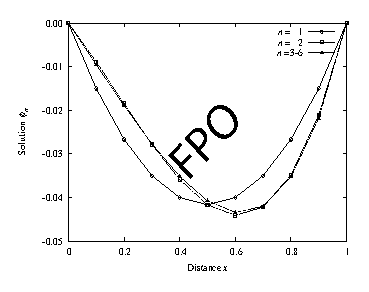
\includegraphics[scale=1]{fpo}
%%\figurebox{10pc}{10pc}[fpo]
\caption{(a) Normalized distribution of $H_T$; (b) Distribution of the
invariant mass of the $e^+$ and reconstructed $\tau^-$pair; (c) Distribution
of the mass of the reconstructed $\zp$; (d) The $5\sigma$ significance contours
in the plane of $m_{\zp}$ and $\sin^2\theta$.
\label{fig:lhc} }
%%%\end{center}
\end{figure}
%\sidecapfalse
%\noindent \underline{\it Flavor changing leptonic interactions}~:~
Flavor-changing leptonic interactions through Higgs exchange are present
in this model, but they are suppressed by lepton masses, as in the original
$A_4$ proposal~\cite{mr01}.  The set of three Higgs doublets $\Phi_i$
transforming as $\underline{3}$ under $T_7$ is rotated by $U$ of Eq.~(1)
to form mass eigenstates $\phi_{0,1,2} \sim 1,\omega,\omega^2$
under the residual $Z_3$, where $\phi_0$ is identified as the one Higgs
doublet (with $\langle \phi_0^0 \rangle = v$) of the Standard Model,
with Yukawa couplings
$v^{-1} [m_e \bar{e}_L e_R + m_\mu \bar{\mu}_L \mu_R + m_\tau
\bar{\tau}_L \tau_R]$, which is of course flavor-conserving.
The ``flavor-changing'' interactions of $\phi_{1,2}$ are then given by
%\bea
%{\cal L}_{int}
%&=& \sqrt{3 \over 2} {g \over M_W} [m_\tau
%\overline{(\nu_\mu,\mu)}_L \tau_R + m_\mu \overline{(\nu_e,e)}_L \mu_R +
%m_e \overline{(\nu_\tau,\tau)}_L e_R] \phi_1 \nonumber \\
%&=& \sqrt{3 \over 2} {g \over M_W} [m_\tau \overline{(\nu_e,e)}_L \tau_R
%+ m_\mu \overline{(\nu_\tau,\tau)}_L \mu_R + m_e \overline{(\nu_\mu,\mu)}_L
%e_R] \phi_2 + H.c.
%\eea
\bea
{\cal L}_{int} = v^{-1} [m_\tau
{\overline{L}_\mu}_L \tau_R + m_\mu {\overline{L}_e}_L \mu_R +
m_e {\overline{L}_\tau}_L e_R] \phi_1 + && \nonumber \\
v^{-1} [m_\tau {\overline{L}_e}_L \tau_R
+ m_\mu {\overline{L}_\tau}_L \mu_R + m_e {\overline{L}_\mu}_L
e_R] \phi_2 + H.c. &&
\eea
However, if the neutrino sector is ignored, a lepton flavor
triality ($Z_3$ symmetry)~\cite{m09} exists here, under which
$e,\mu,\tau \sim 1,\omega^2,\omega$,  implying thus the decays $\tau^+
\to \mu^+ \mu^+ e^-$ and $\tau^+ \to e^+ e^+ \mu^-$, but no others.
In particular, $\mu \to e \gamma$ is forbidden. Using
\[
B(\tau^+ \to \mu^+ \mu^+ e^-) = {m_\tau^2 m_\mu^2 (m_1^2 + m_2^2)^2 \over
m_1^4 m_2^4} B(\tau \to \mu \nu \nu),
\]
the experimental upper limit of $2.3 \times 10^{-8}$ yields the
bound~\cite{m09} $m_1 m_2/\sqrt{m_1^2+m_2^2} > 22$ GeV (174 GeV/$v$)
on the masses of $\psi^0_{1,2} = (\phi^0_1 \pm \bar{\phi}^0_2)/\sqrt{2}$.

%\noindent \underline{\it LHC observations}~:~
Since the Higgs singlets $\chi$ and $\eta$ which support the neutrino
tribimaximal mixing under $T_7$ also transform under $U(1)_{B-L}$, this
model can be tested at the LHC by discovering the
$Z^\prime_{B-L}(\equiv \zp)$ gauge boson.
The partial decay rates of $\zp$ to the usual
quarks and leptons are easily calculated.  Let $\Gamma_0 = g_{B-L}^2 m_{\zp}/12
\pi$, then
$\Gamma_q = (6)(3)(1/3)^2\Gamma_0$, $\Gamma_l = (3)(-1)^2 \Gamma_0$,
$\Gamma_\nu = (3)(-1)^2(1/2)\Gamma_0$.
As for $\zp \to {\psi}^0_{1,2} \bar{\psi}^0_{2,1}$, it has the effective
partial rate $\Gamma_\psi \simeq (2)(-2)^2 \sin^4 \theta (1/4) \Gamma_0$,
where $\sin \theta$ is an effective parameter accounting for the mixing of
$\psi^0_{1,2}$ to $\chi$ and $\eta$ (with the help of a $B-L=0$ singlet $S_i
\sim \underline{3}$). Using Eq.~(18),
we find their signature decays to be given by
\begin{equation}
\psi^0_{1,2} \to \tau^+ \mu^-, ~ \tau^- e^+, ~~~
\bar{\psi}^0_{1,2} \to \tau^- \mu^+, ~ \tau^+ e^-,
\end{equation}
resulting in $\zp$ leptonic final states such as $\tau^- \tau^-
\mu^+ e^+$ for example.  In addition to being crucial for neutrino
tribimaximal mixing to work under $T_7$, the $U(1)_{B-L}$ gauge symmetry
is seen to provide also the means of verifying its predicted interactions.
If the singlet neutrinos $\nu^c_i$ are light enough, they can also be
produced by $\zp$ decay as discussed in Ref.~\cite{hkor08}.  The mass
eigenstates of $\nu^c_i$ are given by Eq.~(13).  Their decays into
$\phi_{1,2}$ and leptons, and the subsequent decays of $\phi_{1,2}$
to leptons (resulting in six leptons in the final state) will then give a
complete picture of tribimaximal mixing in this model.

%\noindent \underline{\it Detailed collider phenomenology}~:~
We now study in detail the process $q\bar{q} \to \zp \to \psi_1 \bar{\psi}_2
+ \psi_2 \bar{\psi}_1$ (assuming $m_1=m_2$)
with the subsequent decays $\psi \to \tau^- e^+$ and $\bar{\psi} \to \tau^-
\mu^+$ at the LHC with $E_{cm} = 14$ TeV.  We consider only the leptonic
decay modes of the $\tau^-$, with branching fraction $17.4\%$ to either
$e^-$ or $\mu^-$.  The collider signature of such events is $e^+ \mu^+
\ell^- \ell^-$ plus missing energy, where $\ell=e,\mu$.  The dominant
backgrounds yielding the same signature are the processes (generated by
MadEvent/MadGraph~\cite{Maltoni:2002qb}):
\bea
&&WWZ: pp\to W^{+}W^{-}Z, W^{\pm}\to \ell^\pm \nu, Z\to \ell^{+}
\ell^{-},  \nonumber \\
&& ZZ: pp\to ZZ, Z\to \ell^+\ell^-,Z\to\tau^+\tau^-,
\tau^\pm\to \ell^{\pm} \nu\bar{\nu},\nonumber\\
&&t\bar{t}: pp\to t\bar{t}\to b(\to \ell^-)\bar{b}(\to \ell^+)W^{+}W^{-},\,
W^{\pm}\to \ell^\pm\nu, \nonumber \\
&& Zb\bar{b}: pp\to Zb(\to \ell^-)\bar{b}(\to \ell^+),\, Z\to\ell^{+}\ell^{-},
\label{eq:smbkgd}
\eea
where $\ell=e,\mu$.
Other SM backgrounds, e.g. $ZZZ$ and $WWWW$, occur at a negligible rate
after kinematic cuts, and are not shown here.
We require no jet tagging and consider only events with both $e^+$ and
$\mu^+$ in the final state.
The first two processes are the irreducible background, while the last two
are reducible as they only contribute when some tagged particles escape
detection, carrying away small transverse momentum ($p_{T}$) or
falling out of the detector rapidity coverage.

Our benchmark points are chosen as follows:
$m_{\zp} = 1000~(1500)~{\rm GeV},~m_{\psi} = 100~(300)~{\rm GeV}$,
$g_{B-L} = g = e/\sin \theta_W$, and $\sin^2\theta = 0.2$.
In our analysis all events are required to pass the following
{\it basic} acceptance cuts:
\bea
& & p_{T,\,\ell}^{(1,2)}\geq 50\,{\rm GeV},
~p_{T,\,\ell}^{(3,4)}\geq 20\,{\rm GeV},
~\left|\eta_{\ell}\right|\leq2.5,
\nonumber \\
& & \Delta R_{\ell\ell^\prime}\geq 0.4,~\met > 30~\rm{GeV},
\label{eq:cut}
\eea
where (1-4) in the superscript index is the $p_T$ order of the charged leptons.
$\Delta R_{ij}$ is the separation in the azimuthal angle ($\phi$)
- pseudorapidity ($\eta$) plane between $i$ and $j$, defined as
$\Delta R_{ij}\equiv \sqrt{\left(\eta_{i}-\eta_{j}\right)^{2}+\left(\phi_{i}-
\phi_{j}\right)^{2}}$.  We also model detector resolution effects by smearing
the final-state energy. To further suppress the SM backgrounds, we demand
\begin{equation}
H_T \equiv \sum_i p_{T,~i} + \met > 300~{\rm GeV}, \label{eq:ht}
\end{equation}
where $i$ denotes the visible particles.
Figure~\ref{fig:lhc}(a) shows the normalized $H_T$ distribution of both signal
and background before the $H_T$ cut. The signal spectrum exhibits an endpoint
around the mass of $\zp$, about 1~TeV, but with a long tail due to the
$\zp$ width and detector smearing effects. Table~\ref{tab:cut} displays
the signal and background cross sections (fb) before and after cuts.
The cut acceptance ($\mathcal{A}_{cut}$) increases with $m_\psi$
as heavy scalar decay generates hard leptons and large $H_T$.
For a light $\psi$ and a heavy $\zp$ (e.g. the benchmark B), $\mathcal{A}_{cut}$
decreases as the two charged leptons from the light scalar decay are
very much parallel and
fail the $\Delta R$ separation cuts.


\begin{table}
\def\a{\hphantom{0}}
\tabcolsep2.9pt
\tbl{Signal and background cross sections (fb) before and after cuts
for four $(m_{\zp},m_\psi)$ (GeV) benchmark points: ($A$) (1000,100), ($B$) (1500,100),
($C$) (1000,300), and ($D$) (1500,300).
The ``no cut'' rates correspond to all leptonic decay modes of $\tau^-$
after $e^+\mu^+$ identification,
the ``basic cut'' and ``$H_T$ cut'' rates are obtained after imposing
Eq.~(\ref{eq:cut}) and Eq.~(\ref{eq:ht}), respectively,
whereas the ``$x_{\tau_i}>0$'' rates are obtained after the $\tau^-$
reconstruction cuts. The bottom row shows the cut acceptance ($\mathcal{A}_{cut}$).
%The ratio of signal to background
%($S/B$) and discovery significance $S/\sqrt{B}$ are calculated
%with an integrated luminosity of $100~{\rm fb}^{-1}$ (which is reduced
%by $\sqrt{10}$ if only 10 fb$^{-1}$ is achieved.)
\label{tab:cut}}{
\begin{tabular}{@{}lcccccccc@{}}
\toprule
              & \tch{(A)}  & \tch{(B)}    & \tch{(C)} & \tch{(D)} & \tch{$t\bar{t}$} & \tch{$WWZ$} & \tch{$ZZ$} & \tch{$Zb\bar{b}$} \\
\colrule
no cut        &5.14  & 0.98\a   &2.57 & 0.72 & 1.22\a   & 0.21\a   & 27.11\a\a   & 2.99\a     \\
basic cut     &1.46  & 0.066  &1.05 & 0.36 & 0.16\a   & 0.02\a   & \a0.0052  & 0.024    \\
$H_T$ cut     &1.41  & 0.065  &1.04 & 0.36 & 0.08\a   & 0.006  & \a0.0\a\a\a     & 0.0\a\a      \\
$x_{\tau}>0$  &0.69  & 0.032  &0.52 & 0.18 & 0.015  & 0.002  & \a0.0\a\a\a     & 0.0\a\a      \\[3pt]
%\hline
$\mathcal{A}_{cut}$&13.4\%  & 3.2\%  & 20\%& 25\% & 1.2\%  & 1\%  & 0.0     & 0.0      \\
\botrule
\end{tabular}}
\end{table}

\begin{figure}[b!]
%%\begin{center}
\includegraphics[scale=0.37]{distro}
%%\figurebox{10pc}{10pc}[distro]
\caption{(a) Normalized distribution of $H_T$; (b) Distribution of the
invariant mass of the $e^+$ and reconstructed $\tau^-$pair; (c) Distribution
of the mass of the reconstructed $\zp$; (d) The $5\sigma$ significance contours
in the plane of $m_{\zp}$ and $\sin^2\theta$.
\label{fig:lhc} }
%%%\end{center}
\end{figure}

To reconstruct the scalar $\psi$, we adopt the collinear approximation
that the charged lepton and neutrinos from $\tau$ decays are parallel
due to the large boost of the $\tau$. Such a condition is satisfied to an
excellent degree because the $\tau$ leptons originate from a heavy scalar
decay in the signal event.  Denoting by $x_{\tau_i}$ the fraction of the parent
$\tau$ energy which each observable decay particle carries, the transverse
momentum vectors are related by~\cite{Rainwater:1998kj}
\be
\vec{\not{\!E}}_T = \left(1/x_{\tau_1} - 1 \right)\vec{p}_1
+\left(1/x_{\tau_2}-1\right)\vec{p}_2. \label{eq:taurec}
\ee
When the decay products are not back-to-back, Eq.~(\ref{eq:taurec}) gives two
conditions for $x_{\tau_i}$ with the $\tau$ momenta as $\vec{p}_1/x_{\tau_1}$
and $\vec{p}_{2}/x_{\tau_2}$, respectively. We further require the calculated
$x_{\tau_i}$ to be positive to remove the unphysical solutions.
%CAO:Since the charged lepton from $\tau^-$ decay could be either $e^-$ or $\mu^-$,
There are two possible combinations of $e^+\ell^-$ clusters
for reconstructing the scalar $\psi$ and gauge boson $\zp$. To
choose the correct combination, we require the $e^+\ell^-$ pairing to be
such that $\Delta R_{e^+\ell^-}$ is minimized.
The mass spectra of the reconstructed $\psi$
and $\zp$ are plotted in
Fig.~\ref{fig:lhc}(b) and (c), respectively, which clearly
display sharp peaks around $m_\psi$ and $m_{Z^\prime}$.
In Fig.~\ref{fig:lhc}(d), we show the $5\sigma$ discovery contours
in the plane of $m_{\zp}$ and $\sin^2\theta$ by requiring 8.5 (5) signal
events for an integration luminosity of $100~(10)~{\rm fb}^{-1}$
respectively. The regions above those curves
are good for discovery.


%\noindent \underline{\it Quark sector}~:~
In the quark sector, if we use $Q_i = (u,d)_i \sim \underline{3}$ and
$u^c_i,d^c_i \sim \underline{1}_i, i =1,2,3$ as we assume for the charged
leptons, we again obtain arbitrary quark masses, but no mixing.
To have realistic mixing angles, the residual $Z_3$ symmetry has to be broken.

%\noindent \underline{\it Conclusion}~:~
Non-Abelian discrete symmetries have been successful in explaining the
tribimaximal mixing of neutrinos, but not their masses.  However, they are
very difficult to
test experimentally. In this paper, by combining $T_7$ and $U(1)_{B-L}$,
we show how a simple renormalizable two-parameter neutrino mass model of
tribimaximal mixing can be constructed, with verifiable experimental
predictions.  The key is the possible discovery of $\zp$ at the TeV
scale, which then decays into neutral Higgs scalars, whose subsequent
exclusive decays into charged leptons have a distinct flavor pattern
which may be observable at the LHC.

\section*{Acknowledgements}
The work of Q.H.C. is supported in part by the U.~S.~Dept.~of Energy
Grant No.~DE-AC02-06CH11357 and in part
by the Argonne National Lab.~and Univ.~of Chicago Joint Theory Institute
Grant No.~03921-07-137.
The work of S.K. and H.O. is supported in part by the Science and Technology
Development Fund (STDF) Project ID 437 and the ICTP Project ID 30.
The work of E.M. is supported in part by the U.~S.~Dept.~of Energy
Grant No. DE-FG03-94ER40837.


%\newpage
\bibliographystyle{unsrt}
\begin{thebibliography}{99}
\bibitem{doshi2017} Doshi-Velez, Finale, and Been Kim. "Towards a rigorous science of interpretable machine learning." arXiv preprint arXiv:1702.08608 (2017).
\bibitem{linardatos2021} Linardatos, Pantelis, Vasilis Papastefanopoulos, and Sotiris Kotsiantis. "Explainable AI: A review of machine learning interpretability methods." Entropy 23.1 (2021): 18.
\bibitem{lake2015} Lake, Brenden M., Ruslan Salakhutdinov, and Joshua B. Tenenbaum. "Human-level concept learning through probabilistic program induction." Science 350.6266 (2015): 1332-1338.
\bibitem{nanayakkara2018}Nanayakkara, Shane, et al. "Characterising risk of in-hospital mortality following cardiac arrest using machine learning: A retrospective international registry study." PLoS medicine 15.11 (2018): e1002709.
\bibitem{wu2021} Wu, Leihong, et al. "Trade-off Predictivity and Explainability for Machine-Learning Powered Predictive Toxicology: An in-Depth Investigation with Tox21 Data Sets." Chemical Research in Toxicology 34.2 (2021): 541-549.

\bibitem{mr01} E. Ma and G. Rajasekaran, Phys. Rev. {\bf D64}, 113012 (2001).
\bibitem{m04} E. Ma, Phys. Rev. {\bf D70}, 031901 (2004).
\bibitem{SNO} B. Aharmim {\it et al.}, Phys. Rev. {\bf C72}, 055502 (2005).
\bibitem{ikoost10} For a recent review, see for example H. Ishimori,
T. Kobayashi, H. Ohki, H. Okada, Y. Shimizu, and M. Tanimoto,
Prog. Theor. Phys. Suppl. {\bf 183}, 1 (2010).
\bibitem{af10} For a recent review, see for example G. Altarelli and F.
Feruglio, Rev. Mod. Phys. {\bf 82}, 2701 (2010).
\bibitem{af05} G. Altarelli and F. Feruglio, Nucl. Phys. {\bf B720}, 64 (2005).
\bibitem{bh05} K. S. Babu and X.-G. He, hep-ph/0507217 (2005).
\bibitem{c78} N. Cabibbo, Phys. Lett. {\bf 72}, 333 (1978).
\bibitem{w78} L. Wolfenstein, Phys. Rev. {\bf D18}, 958 (1978).
\bibitem{m10-1} E. Ma, Mod. Phys. Lett. {\bf A25}, 2215 (2010).
\bibitem{m06-1} E. Ma, Mod. Phys. Lett. {\bf A21}, 2931 (2006).
\bibitem{ms98} E. Ma and U. Sarkar, Phys. Rev. Lett. {\bf 80}, 5716 (1998).

%\bibitem{lnr07} C. Luhn, S. Nasri, and P. Ramond, Phys. Lett. {\bf B652}, 27
%(2007).
%\bibitem{hss09} C. Hagedorn, M. A. Schmidt, and A. Yu. Smirnov, Phys. Rev.
%{\bf D79} 036002 (2009).
%\bibitem{kl09} S. F. King and C. Luhn, JHEP {\bf 0910}, 093 (2009).
\bibitem{lnr07} C. Luhn, S. Nasri, and P. Ramond, Phys. Lett. {\bf B652}, 27
(2007); C. Hagedorn, M. A. Schmidt, and A. Yu. Smirnov, Phys. Rev.
{\bf D79} 036002 (2009); S. F. King and C. Luhn, JHEP {\bf 0910}, 093 (2009).

\bibitem{hkor08} See for example K. Huitu, S. Khalil, H. Okada, and S. K. Rai,
Phys. Rev. Lett. {\bf 101}, 181802 (2008).

%\bibitem{m06-2} E. Ma, Mod. Phys. Lett. {\bf A21}, 1917 (2006).
%\bibitem{mvkr07} I. de Medeiros Varzielas, S. F. King, and G. G. Ross,
%Phys. Lett. {\bf B648}, 201 (2007).
%\bibitem{m08} E. Ma, Phys. Lett. {\bf B660}, 505 (2008).

\bibitem{m06-2} E. Ma, Mod. Phys. Lett. {\bf A21}, 1917 (2006);
I. de Medeiros Varzielas, S. F. King, and G. G. Ross,
Phys. Lett. {\bf B648}, 201 (2007); E. Ma, Phys. Lett. {\bf B660}, 505 (2008).


%\bibitem{l07} C. S. Lam, Phys. Lett. {\bf B656}, 193 (2007).
%\bibitem{bhl08} A. Blum, C. Hagedorn, and M. Lindner, Phys. Rev. {\bf D77},
%076004 (2008).

\bibitem{l07} C. S. Lam, Phys. Lett. {\bf B656}, 193 (2007);
A. Blum, C. Hagedorn, and M. Lindner, Phys. Rev. {\bf D77}, 076004 (2008).


%\bibitem{m09} E. Ma, Phys. Lett. {\bf B671}, 366 (2009).
%\bibitem{m10-2} E. Ma, Phys. Rev. {\bf D82}, 037301 (2010).

\bibitem{m09} E. Ma, Phys. Lett. {\bf B671}, 366 (2009); E. Ma, Phys. Rev. {\bf D82}, 037301 (2010).


%\bibitem{klm09} S. Khalil, H.-S. Lee, and E. Ma, Phys. Rev. {\bf D79},
%041701(R) (2009).
%\bibitem{klm10} S. Khalil, H.-S. Lee, and E. Ma, Phys. Rev. {\bf D81},
%051702(R) (2010).
%\cite{Maltoni:2002qb}
\bibitem{Maltoni:2002qb}
  F.~Maltoni and T.~Stelzer,
  %``MadEvent: Automatic event generation with MadGraph,''
  JHEP {\bf 0302}, 027 (2003).
  %[arXiv:hep-ph/0208156].
  %%CITATION = JHEPA,0302,027;%%
%\cite{Rainwater:1998kj}
\bibitem{Rainwater:1998kj}
  D.~L.~Rainwater, D.~Zeppenfeld and K.~Hagiwara,
  %``Searching for H --> tau tau in weak boson fusion at the LHC,''
  Phys.\ Rev.\  D {\bf 59}, 014037 (1999).
  %[arXiv:hep-ph/9808468].
  %%CITATION = PHRVA,D59,014037;%%
\end{thebibliography}

\end{document}






